\chapter{โครงสร้างข้อมูลพื้นฐาน (Data Structure)}

ไลบรารีแม่แบบมาตรฐาน (Standard Template Library : STL) เป็นไลบรารีของภาษา C++ ประกอบไปด้วยขั้นตอนวิธี คอนเทนเนอร์ และอีกมากมาย ซึ่งในบทนี้จะกล่าวถึงเพียงบางชนิดเท่านั้น และโครงสร้างข้อมูลที่ปรากฏในบทนี้เป็นเพียงโครงสร้างข้อมูลพื้นฐานที่ควรรู้จัก เพื่อใช้ในการแก้ปัญหาต่างๆ ได้ง่ายยิ่งขึ้น

\section{รายการโยง (Linked list)}

Linked list เป็นโครงสร้างข้อมูลแบบเส้นที่ข้อมูลไม่ได้ถูกเก็บไว้ในหน่วยความจำแบบเรียงติดกัน แต่ถูกเชื่อมโยงโดยตัวชี้ (Pointer)

\begin{figure}[h!]
    \centering
    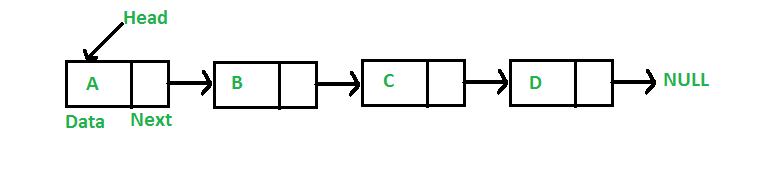
\includegraphics[width=13cm]{images/list-pointer}
    \caption{การเชื่อมโยงโดยใช้ Pointer}
    \label{fig:list-pointer}
\end{figure}
จากรูป 5.1 จะเห็นได้ว่า ใน Linked list จะประกอบไปด้วยโหนด (กลุ่มของข้อมูลและตัวชี้)

ข้อดีของ Linked list คือการจัดการข้อมูล ได้แก่ การเพิ่ม/ลบข้อมูล สามารถกระทำได้โดยการนำโหนดเข้ามาแทรก หรือนำโหนดออกไปได้ทันที จึงใช้เวลาการทำงาน $O(1)$ ซึ่งถ้าใช้ Array ในการจัดการข้อมูล การลบหรือเพิ่มข้อมูลต้องใช้เวลาการทำงาน $O(n)$ เลยทีเดียว (การเพิ่ม/ลบระหว่างข้อมูลในอาเรย์ ต้องทำการเลื่อนข้อมูลทั้งหมดที่อยู่หลังข้อมูลที่จะแทรกด้วย)

ข้อเสียของ  Linked list คือ เนื่องจากการเก็บข้อมูลที่ไม่ได้เรียงต่อเนื่องในหน่วยความจำ การเข้าถึงข้อมูลของ Linked list จึงเป็นไปได้ยาก คือต้องทำการไล่ค้นหาจากโหนด Head ไปเรื่อยๆ ($O(n)$) ไม่สามารถระบุเป็นหมายเลขของโหนดได้ แตกต่างจาก Array ที่สามารถระบุหมายเลขของข้อมูลได้ทันที ($O(1)$)

ในการเรียกใช้ สามารถเรียกใช้ STL ที่ชื่อว่า \texttt{list} ได้ โดยระบุประเภทของข้อมูลต้องการเก็บด้วย เช่น \texttt{list<int > listName;}

\subsection{Singly Linked list}

Singly Linked list เป็น Linked list ที่แต่ละโหนดมีตัวชี้ไปทางเดียว คือชี้ไปยังตัวต่อไปไม่มีการชี้กลับไปยังตัวก่อนหน้า โดยมีโหนดแรกเรียกว่า Head และโหนดสุดท้ายชี้ต่อไปยัง null (null เปรียบเป็นช่องว่าง หมายความว่าไม่มีโหนดต่อไปอีกแล้ว) 

\begin{figure}[h!]
    \centering
    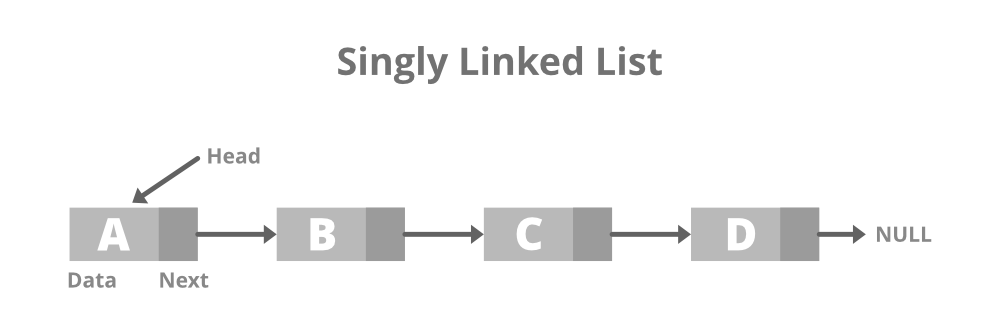
\includegraphics[width=12cm]{images/singly-list}
    \caption{Singly Linked List}
    \label{fig:singly-list}
\end{figure}

\subsection{Circular Linked list}

Circular Linked list เป็น Linked list ที่แต่ละโหนดมีตัวชี้ไปทางเดียวเหมือนกับ Singly Linked list แตกต่างกันที่โหนดสุดท้ายไม่ได้ชี้ไปที่ null แต่ชี้ไปที่โหนด Head แทน ทำให้เกิดเป็นวงขึ้น

\begin{figure}[h!]
    \centering
    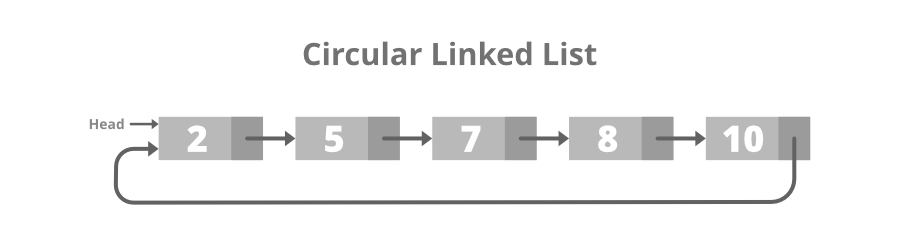
\includegraphics[width=12cm]{images/circular-list}
    \caption{Circular Linked List}
    \label{fig:circular-list}
\end{figure}

\subsection{Doubly Linked list}

Doubly Linked list เป็น Linked list ที่แต่ละโหนดมีตัวชี้ 2 ทิศทางคือ ชี้ไปยังตัวถัดไปและชี้กลับไปยังตัวก่อนหน้า โดยโหนด Head จะชี้ไปยังโหนดถัดไปและ null และโหนดสุดท้ายจะชี้ไปยัง null และโหนดก่อนหน้า

\begin{figure}[h!]
    \centering
    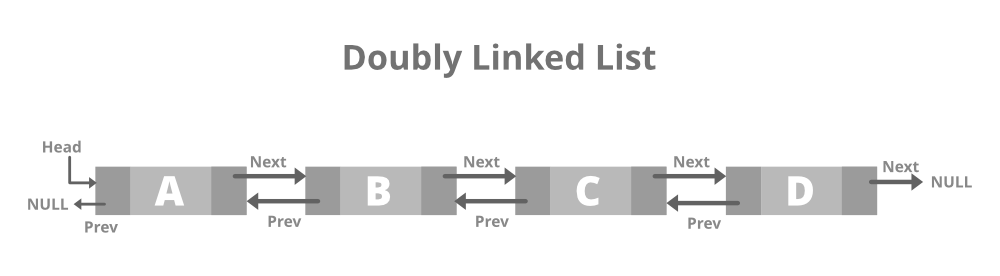
\includegraphics[width=12cm]{images/doubly-list}
    \caption{Doubly Linked List}
    \label{fig:doubly-list}
\end{figure}

\section{กองซ้อน (Stack)}

กองซ้อนเป็นโครงสร้างข้อมูลแบบเส้นที่มีหลักการทำงานแบบ Last In First Out (LIFO) หมายความว่าหากต้องการลบข้อมูล ข้อมูลที่ถูกแทรกเข้ามาล่าสุดจะถูกลบก่อน อาจมองเป็นกองกระดาษที่ซ้อนกันอยู่ หากจะเอาออกก็ต้องดึงใบข้างบนออกก่อน

\begin{figure}[h!]
    \centering
    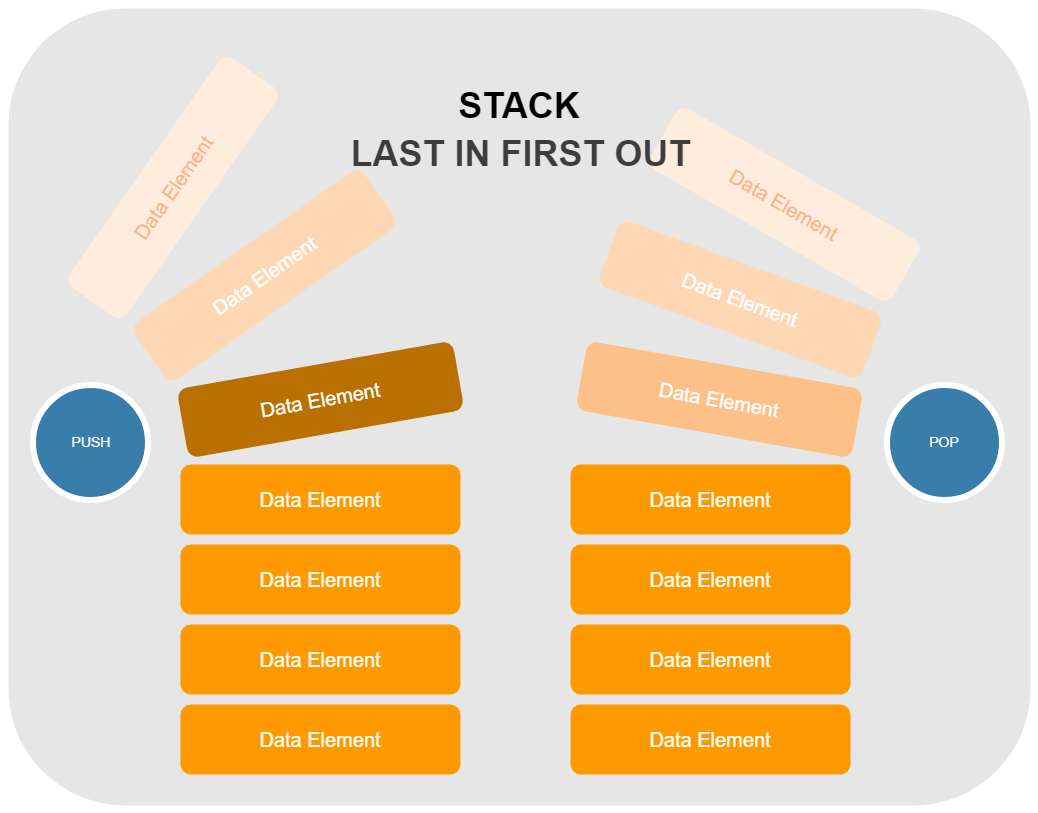
\includegraphics[width=13cm]{images/stack_LIFO}
    \caption{Stack}
    \label{fig:stack}
\end{figure}

ในการเรียกใช้ สามารถเรียกใช้ STL ที่ชื่อว่า \texttt{stack} ได้ โดยระบุประเภทของข้อมูลต้องการเก็บด้วย เช่น \texttt{stack<int > stackName;}

คำสั่งพื้นฐานของ stack ที่ใช้บ่อย มีดังนี้
\begin{itemize}
\item push() เป็นคำสั่งที่ใช้ในการเพิ่มข้อมูลลงไปด้านบนสุดใน stack ($O(1)$)
\item pop() เป็นคำสั่งที่ใช้ในการลบข้อมูลด้านบนสุดออกจาก stack ($O(1)$)
\item empty() เป็นคำสั่งที่ใช้ในการตรวจสอบว่า stack ว่างหรือไม่ ($O(1)$)
\item size() เป็นคำสั่งที่ใช้ในการตรวจสอบขนาดของ stack ว่ามีข้อมูลอยู่เท่าใด ($O(1)$)
\item top() เป็นคำสั่งที่ใช้ในการอ้างอิงข้อมูลไปยังข้อมูลบนสุดของ stack ($O(1)$)
\end{itemize}

\newpage

\subsection{Infix Prefix Postfix}

\begin{itemize}
\item \textbf{Infix} คือรูปแบบนิพจน์โดยทั่วไป เช่น $A * ( B + C ) / D$
\item \textbf{Prefix} คือรูปแบบนิพจน์ที่ตัวดำเนินการ (Operator) ถูกเขียนก่อนตัวถูกดำเนินการ (Operand) เช่น $/ * A + B C D$
\item \textbf{Postfix} คือรูปแบบนิพจน์ที่ตัวถูกดำเนินการ (Operand) ถูกเขียนก่อนตัวดำเนินการ (Operator) เช่น $A B C + * D /$
\end{itemize}

\textbf{หมายเหตุ:} Operator ได้แก่ การดำเนินการทางคณิตศาสตร์ต่างๆ เช่น $+$, $-$, $*$, $/$ เป็นต้น และ Operand ได้แก่ตัวเลขหรือตัวแปรต่างๆ เช่น $10$, $k$ เป็นต้น

หนึ่งในประโยชน์ของ stack คือการเปลี่ยน Infix เป็น Postfix

\subsubsection{Infix to Postfix}

การเปลี่ยน Infix เป็น Postfix มีขั้นตอนหลักๆ ดังนี้
\begin{enumerate}
\item ถ้าเป็น Operand ให้แสดงผลออกมาได้เลย
\item ถ้าเป็น Operator ให้พิจารณา stack
		\begin{enumerate}
\item ถ้าตัวที่จะใส่เป็นเครื่องหมายวงเล็บปิด `)' ให้แสดงผลตัวบนสุดของ stack และเอาออกไปจนกว่าจะเจอวงเล็บเปิด `('
\item ถ้าตัวบนสุดมีค่าความสำคัญไม่น้อยกว่าตัวที่จะใส่ ให้แสดงผลตัวบนสุดนั้น และเอาออกจาก stack (ทำซำ้จนกว่าจะใส่ได้)
\item ไม่เช่นนั้น ให้ใส่ลงไปได้เลย
		\end{enumerate}
\end{enumerate}



\section{แถวคอย (Queue)}

แถวคอยเป็นโครงสร้างข้อมูลแบบเส้นที่มีหลักการทำงานแบบ First In First Out (FIFO) หมายความว่าข้อมูลที่เข้ามาก่อนจะได้ออกก่อน เหมือนกับการยืนเข้าแถว คนที่เข้าแถว (enqueue) ก่อนจะได้ออกจากแถว (dequeue) ก่อน

\begin{figure}[h!]
    \centering
    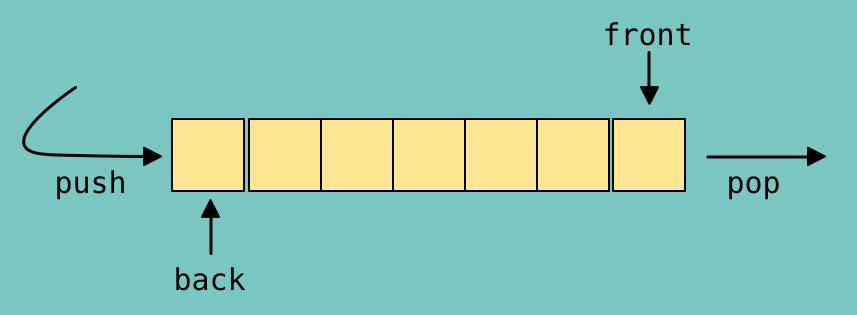
\includegraphics[width=13cm]{images/queue}
    \caption{Queue}
    \label{fig:queue}
\end{figure}
ในการเรียกใช้ สามารถเรียกใช้ STL ที่ชื่อว่า \texttt{queue} ได้ โดยระบุประเภทของข้อมูลต้องการเก็บด้วย เช่น \texttt{queue<int > queueName;}

คำสั่งพื้นฐานของ stack ที่ใช้บ่อย มีดังนี้
\begin{itemize}
\item push() เป็นคำสั่งที่ใช้ในการเพิ่มข้อมูลลงไปต่อท้ายใน queue ($O(1)$)
\item pop() เป็นคำสั่งที่ใช้ในการลบข้อมูลด้านหน้าสุดออกจาก queue ($O(1)$)
\item empty() เป็นคำสั่งที่ใช้ในการตรวจสอบว่า queue ว่างหรือไม่ ($O(1)$)
\item size() เป็นคำสั่งที่ใช้ในการตรวจสอบขนาดของ queue ว่ามีข้อมูลอยู่เท่าใด ($O(1)$)
\item front() เป็นคำสั่งที่ใช้ในการอ้างอิงข้อมูลที่อยู่ด้านหน้าสุดของ queue ($O(1)$)
\item back() เป็นคำสั่งที่ใช้ในการอ้างอิงข้อมูลที่อยู่ด้านท้ายสุดของ queue ($O(1)$)
\end{itemize}

\section{ตารางแฮช (Hash Table)}

ตารางแฮชเป็นโครงสร้างข้อมูลแบบตาราง ใช้ในการเก็บข้อมูลจำนวนมาก เพื่อความสะดวกต่อการเก็บและค้นหาผ่านฟังก์ชั่นแฮช (Hash function)

ข้อมูลที่นำมามาเก็บในตารางแฮชต้องผ่านฟังก์ชั่นแฮชให้กลายเป็น key ก่อนเสมอ key ที่ได้ออกมาจะมีความจำเพาะต่อข้อมูลนั้น แล้วจึงจะสามารถนำไปเก็บในตารางได้

ข้อดีของตารางแฮช คือ หากฟังก์ชั่นแฮชมีประสิทธิภาพ จน key ที่ได้จากแต่ละข้อมูลแตกต่างกัน การค้นหาและการเพิ่มลดสมาชิกจะใช้เวลาการทำงานคงที่ ($O(1)$)

ในการเรียกใช้ สามารถเรียกใช้ STL ที่ชื่อว่า \texttt{hash} ได้ โดยระบุประเภทของข้อมูลต้องการเก็บด้วย เช่น \texttt{hash<string > hashName;}

\subsection{การชนกันของข้อมูล (Collision)}

ในบางครั้ง ฟังก์ชั่นแฮชที่ไม่มีประสิทธิภาพมากพอ จะทำให้ 2 ข้อมูลที่แตกต่างกันมี key เดียวกันได้ จึงต้องมีการแก้ปัญหาการชนของข้อมูล วิธีแก้ปัญหาที่จะแนะนำคือ วิธี Open Addressing ซึ่งเป็นการกระโดดจากที่เดิมเป็นระยะฟังก์ชั่นหนึ่ง จนกว่าจะเจอช่องว่างให้ใส่ key ลงไปได้

\subsubsection{การตรวจเชิงเส้น (Linear Probing)}

การตรวจเชิงเส้นจะทำให้การกระโดดมีระยะคงที่ และทำให้ข้อมูลเกาะกลุ่มกันเป็นกลุ่มใหญ่ แต่มีจำนวนกลุ่มน้อย ทำให้ถ้ามีการชนบริเวณนี้จะต้องใช้เวลามากในการกระโดดให้พ้นช่วงการเกาะกลุ่มของข้อมูลนี้

\subsubsection{การตรวจกำลังสอง (Quadratic Probing)}

การตรวจกำลังสองจะทำให้การกระโดดมีระยะเป็นฟังก์ชั่นตรรกยะ (ซึ่งมักเป็นฟังก์ชั่นกำลังสอง) การกระโดดเช่นนี้จะทำให้ข้อมูลติดกันเป็นกลุ่มขนาดเล็ก แต่มีจำนวนกลุ่มมาก ซึ่งการกระโดดแบบนี้ อาจทำให้บางช่องว่างไม่ถูกเจอเลยก็เป็นได้

\section{แถวคอยลำดับความสำคัญ (Priority queue / Heap)}

Heap เป็นโครงสร้างข้อมูลแบบต้นไม้ที่มีหลักการจาก Binary heap (อาจใช้หลักการอื่น เช่น Fibonacci heap ได้ แต่ในบทนี้จะกล่าวถึงแค่ Binary heap) โดยความสัมพันธ์ที่สำคัญระหว่างปมพ่อและปมลูกคือ ปมพ่อต้องมีความสำคัญมากกว่าปมลูกเสมอ

\begin{figure}[h!]
    \centering
    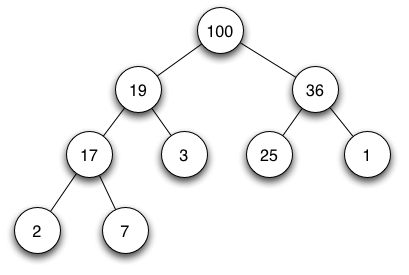
\includegraphics[width=13cm]{images/max-heap}
    \caption{Heap ที่กำหนดให้ความสำคัญขึ้นกับค่าของปม}
    \label{fig:max-heap}
\end{figure}
Heap เป็นต้นไม้ที่มีการปรับแต่งอยู่เสมอหากมีข้อมูลเข้าหรือออก ทำให้ต้นไม้ที่ได้เป็นต้นไม้รับประกันความสูง จึงรับประกันได้ว่าเวลาการทำงานในการเพิ่ม/ลบข้อมูลจะเป็น $O(log(n))$ เสมอ และการเข้าถึงข้อมูลที่สำคัญที่สุดสามารถทำได้ใน  $O(1)$

ในการเรียกใช้ สามารถเรียกใช้ STL ที่ชื่อว่า \texttt{priority\_queue} ได้ โดยระบุประเภทของข้อมูลต้องการเก็บด้วย เช่น \texttt{priority\_queue<int > heapName;} โดยทั่วไป Heap ที่ได้จะเป็นประเภท Max heap คือให้ความสำคัญขึ้นกับค่าของข้อมูล หากข้อมูลมีค่ามากก็จะมีความสำคัญมากตามไปด้วย

\subsection{การเพิ่มข้อมูล}

การเพิ่มข้อมูลใน Heap ทำได้โดยนำปมข้อมูลนั้นไปต่อท้าย แล้วตรวจสอบว่ามีความสำคัญมากกว่าปมพ่อหรือไม่ หากมากกว่าจึงสลับระหว่างปมนั้นๆ กับปมพ่อไปเรื่อยๆ จนปมพ่อมีความสำคัญมากกว่าปมลูก เรียกว่า Heapify up

\subsection{การลบข้อมูลที่สำคัญที่สุด}

การลบข้อมูลทำได้โดยการดึงเอาข้อมูลที่เป็นปมรากออก และนำปมสุดท้าย (ความสำคัญน้อย) มาแทน แล้วจึงค่อยๆ สลับกับปมลูกจนปมลูกมีความสำคัญน้อยกว่าปมพ่อ แล้วจึงหยุด 
เรียกว่า Heapify down

\section{เซตไม่มีส่วนร่วม (Disjoint Set)}

Disjoint set เป็นโครงสร้างข้อมูลที่ใช้เก็บเซตที่ไม่มีส่วนร่วมกันเลย และมีประโยชน์ใน Union-Find algorithm ซึ่งเป็นขั้นตอนวิธีที่ดำเนิการบนโครงสร้างข้อมูลนี้

\subsection{Union-Find algorithm}

ขั้นตอนวิธีนี้ สามารถใช้ในการรวมระหว่าง 2 เซตเข้าด้วยกัน หรือตรวจสอบว่าสมาชิก 2 ตัวใดๆ อยู่ในเซตเดียวกันหรือไม่

อาเรย์ \texttt{p} ใช้บอกปมพ่อของสมาชิกแต่ละตัว ในตอนเริ่มต้นกำหนดให้สมาชิกแต่ละตัวมีปมพ่อเป็นตัวเอง คือ \texttt{p[i] = i} เมื่อ i คือสมาชิกแต่ละตัว

\begin{figure}[h!]
    \centering
    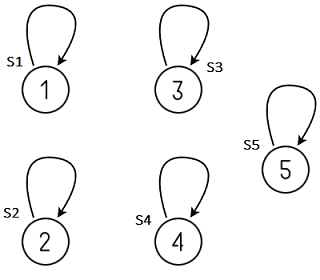
\includegraphics[width=13cm]{images/union-find-init}
    \caption{การกำหนดปมพ่อให้สมาชิกแต่ละตัวเป็นตัวเอง}
    \label{fig:union-find-init}
\end{figure}

\newpage

หลังจากนั้น หากมีการรวมเซตของ 3 กับ 4 เข้าด้วยกัน เราสามารถกล่าวได้ว่าปมพ่อของ 4 คือ 3 (หรือกระทำได้ในทางกลับกัน คือให้ปมพ่อของ 3 เป็น 4 ก็ได้เช่นกัน) จะได้ว่ารากของ 3 และ 4 เป็นรากเดียวกันคือ 3

\begin{figure}[h!]
    \centering
    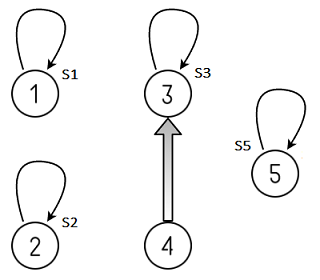
\includegraphics[width=13cm]{images/union-find-3-4}
    \caption{การเชื่อมเซตของ 3 และ 4}
    \label{fig:union-find-3-4}
\end{figure}

การตรวจหาราก (Find root) สามารถทำได้ด้วยฟังก์ชั่นนี้
\begin{lstlisting}
int findRoot(int current) {
	if(p[current] == current)
    	return current;
    return findRoot(p[current]);
}
\end{lstlisting}
ฟังก์ชั่นนี้จะทำการตรวจสอบปมพ่อว่าเป็นปมตัวเองหรือไม่ หากเป็นแสดงว่าปมนั้นๆ เป็นปมรากแล้ว หากยังไม่เป็นจึงทำการตรวจสอบปมพ่อต่อไป การทำงานของฟังก์ชั่นนี้จะใช้เวลา $O(n)$ ซึ่งสามารถใช้เทคนิค \textbf{Path Compression} ลดเวลาการทำงานให้เหลือ $O(log(n))$ ได้

\begin{lstlisting}
int findRoot(int current) {
	if(p[current] == current)
    	return current;
    return p[current] = findRoot(p[current]);
}
\end{lstlisting}
Path Compression เป็นเทคนิคที่ใช้ลดเวลาการค้นหาของการตรวจสอบครั้งถัดไป จะเห็นได้ว่ามีความแตกต่างเพียงแค่บรรทัดที่ 4 เทคนิคนี้จะเป็นการเปลี่ยนปมพ่อของทุกปมที่อยู่ระหว่างการตรวจสอบให้มีปมพ่อเป็นปมรากทั้งหมด (ลดระยะทางการค้นหาปมรากในแต่ละครั้งได้)
